\documentclass[usenames,dvipsnames,table]{beamer}

%% Packages
\usepackage{soul}
\usepackage{xcolor}
\usepackage{listings}
\usepackage{booktabs}
%% -- 

%% Beamer theme and options
% \usetheme[numbering=fullbar]{focus}
% \setbeamercovered{transparent}
\usetheme{Arguelles}
\setbeamertemplate{caption}{\raggedright\insertcaption\par}
%% --

%% Titlepage
\title{YouTube spam detection}
\subtitle{Artificial Intelligence for CyberSecurity}
\author{Alessandro Zanatta}
\institute{University of Pisa}
% \logo{\includegraphics[height=1.2cm]{./logos/unipi}}
\addtobeamertemplate{title page}{}{}
%% -- 

%% Commands
% Simple highlighting
\newcommand<>{\myhl}[1]{\alert#2{\hl#2{#1}}}

% Remove logo on certain slides
\newcommand{\nologo}{\setbeamertemplate{logo}{}}

% Ignore margins when needed
\newcommand\Wider[2][3em]{%
	\makebox[\linewidth][c]{%
		\begin{minipage}{\dimexpr\textwidth+#1\relax}
			\raggedright#2
		\end{minipage}%
	}%
}
%% -- 

\begin{document}

\frame{\titlepage}

\section{Introduction}
\begin{frame}
	\frametitle{Dataset and goal}

	Total of 1956 YouTube comments from 5 different (famous) musical
	videos\footnote{\href{https://archive.ics.uci.edu/dataset/380/youtube+spam+collection}{https://archive.ics.uci.edu/dataset/380/youtube+spam+collection}}
	with the following features:
	\begin{itemize}
		\item Comment ID
		\item Author
		\item Date
		\item Content
		\item Class
	\end{itemize} \pause

	\myhl{Goal:} recognize and differentiate between legitimate (ham) comments and spam comments!
\end{frame}

\section{Data exploration}
\begin{frame}
	\frametitle{Example entries}
	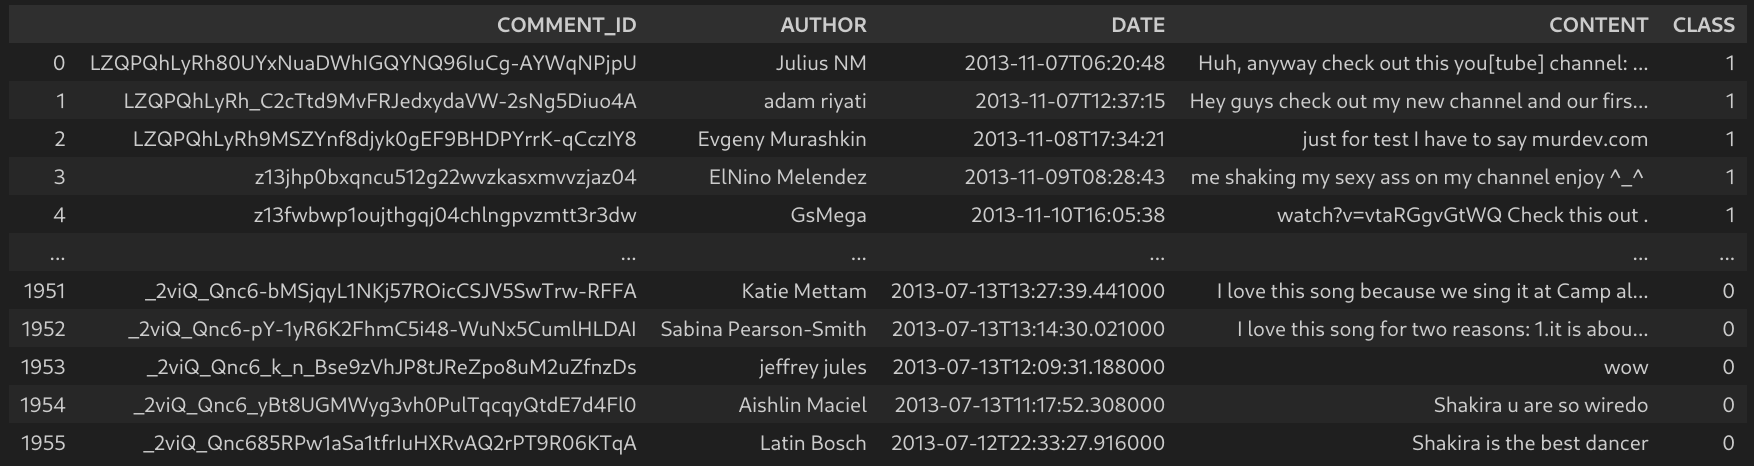
\includegraphics[width=\textwidth]{../src/figures/example_entries}

	Class equal to one indicates spam!
\end{frame}

\begin{frame}
	\frametitle{Word cloud}
	\begin{figure}[ht]
		\begin{minipage}[b]{0.45\linewidth}
			\centering
			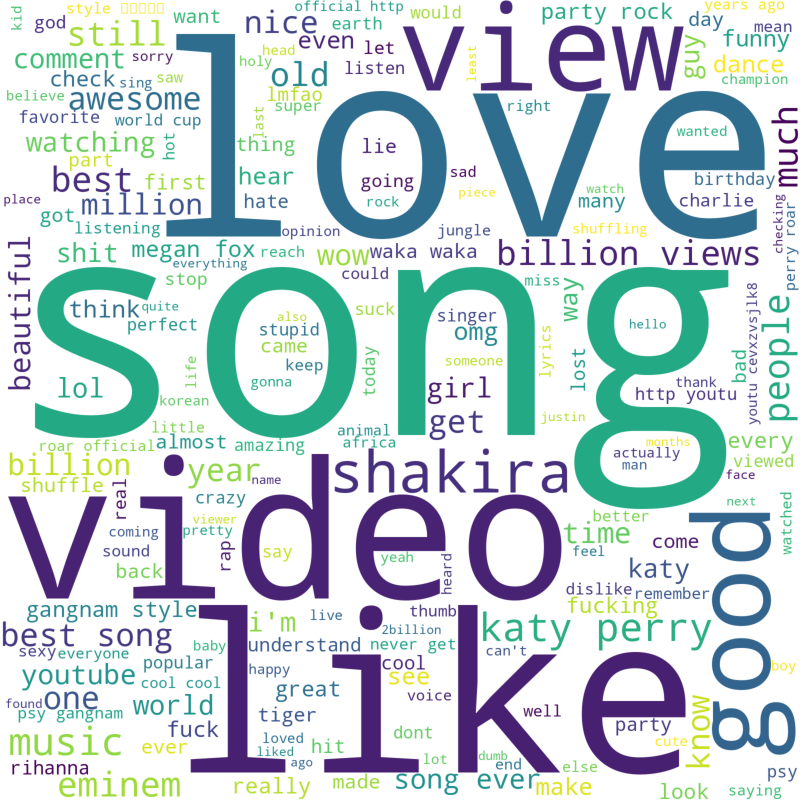
\includegraphics[width=\textwidth]{../src/figures/ham_wordcloud}
			\caption{Ham word cloud}
		\end{minipage}
		\hspace{0.05\textwidth}
		\begin{minipage}[b]{0.45\linewidth}
			\centering
			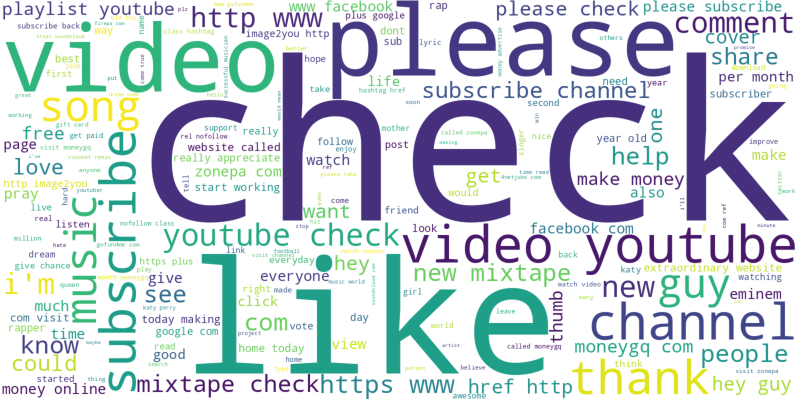
\includegraphics[width=\textwidth]{../src/figures/spam_wordcloud}
			\caption{Spam word cloud}
		\end{minipage}
	\end{figure}
\end{frame}

\begin{frame}
	\frametitle{Most frequent words}

	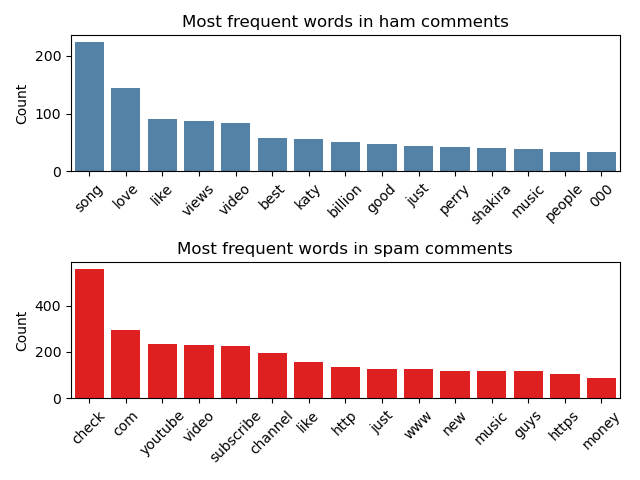
\includegraphics[width=\textwidth]{../src/figures/word_frequencies}
\end{frame}

\begin{frame}
	\frametitle{Balanced dataset}

	Classes are (basically) balanced!

	\centering
	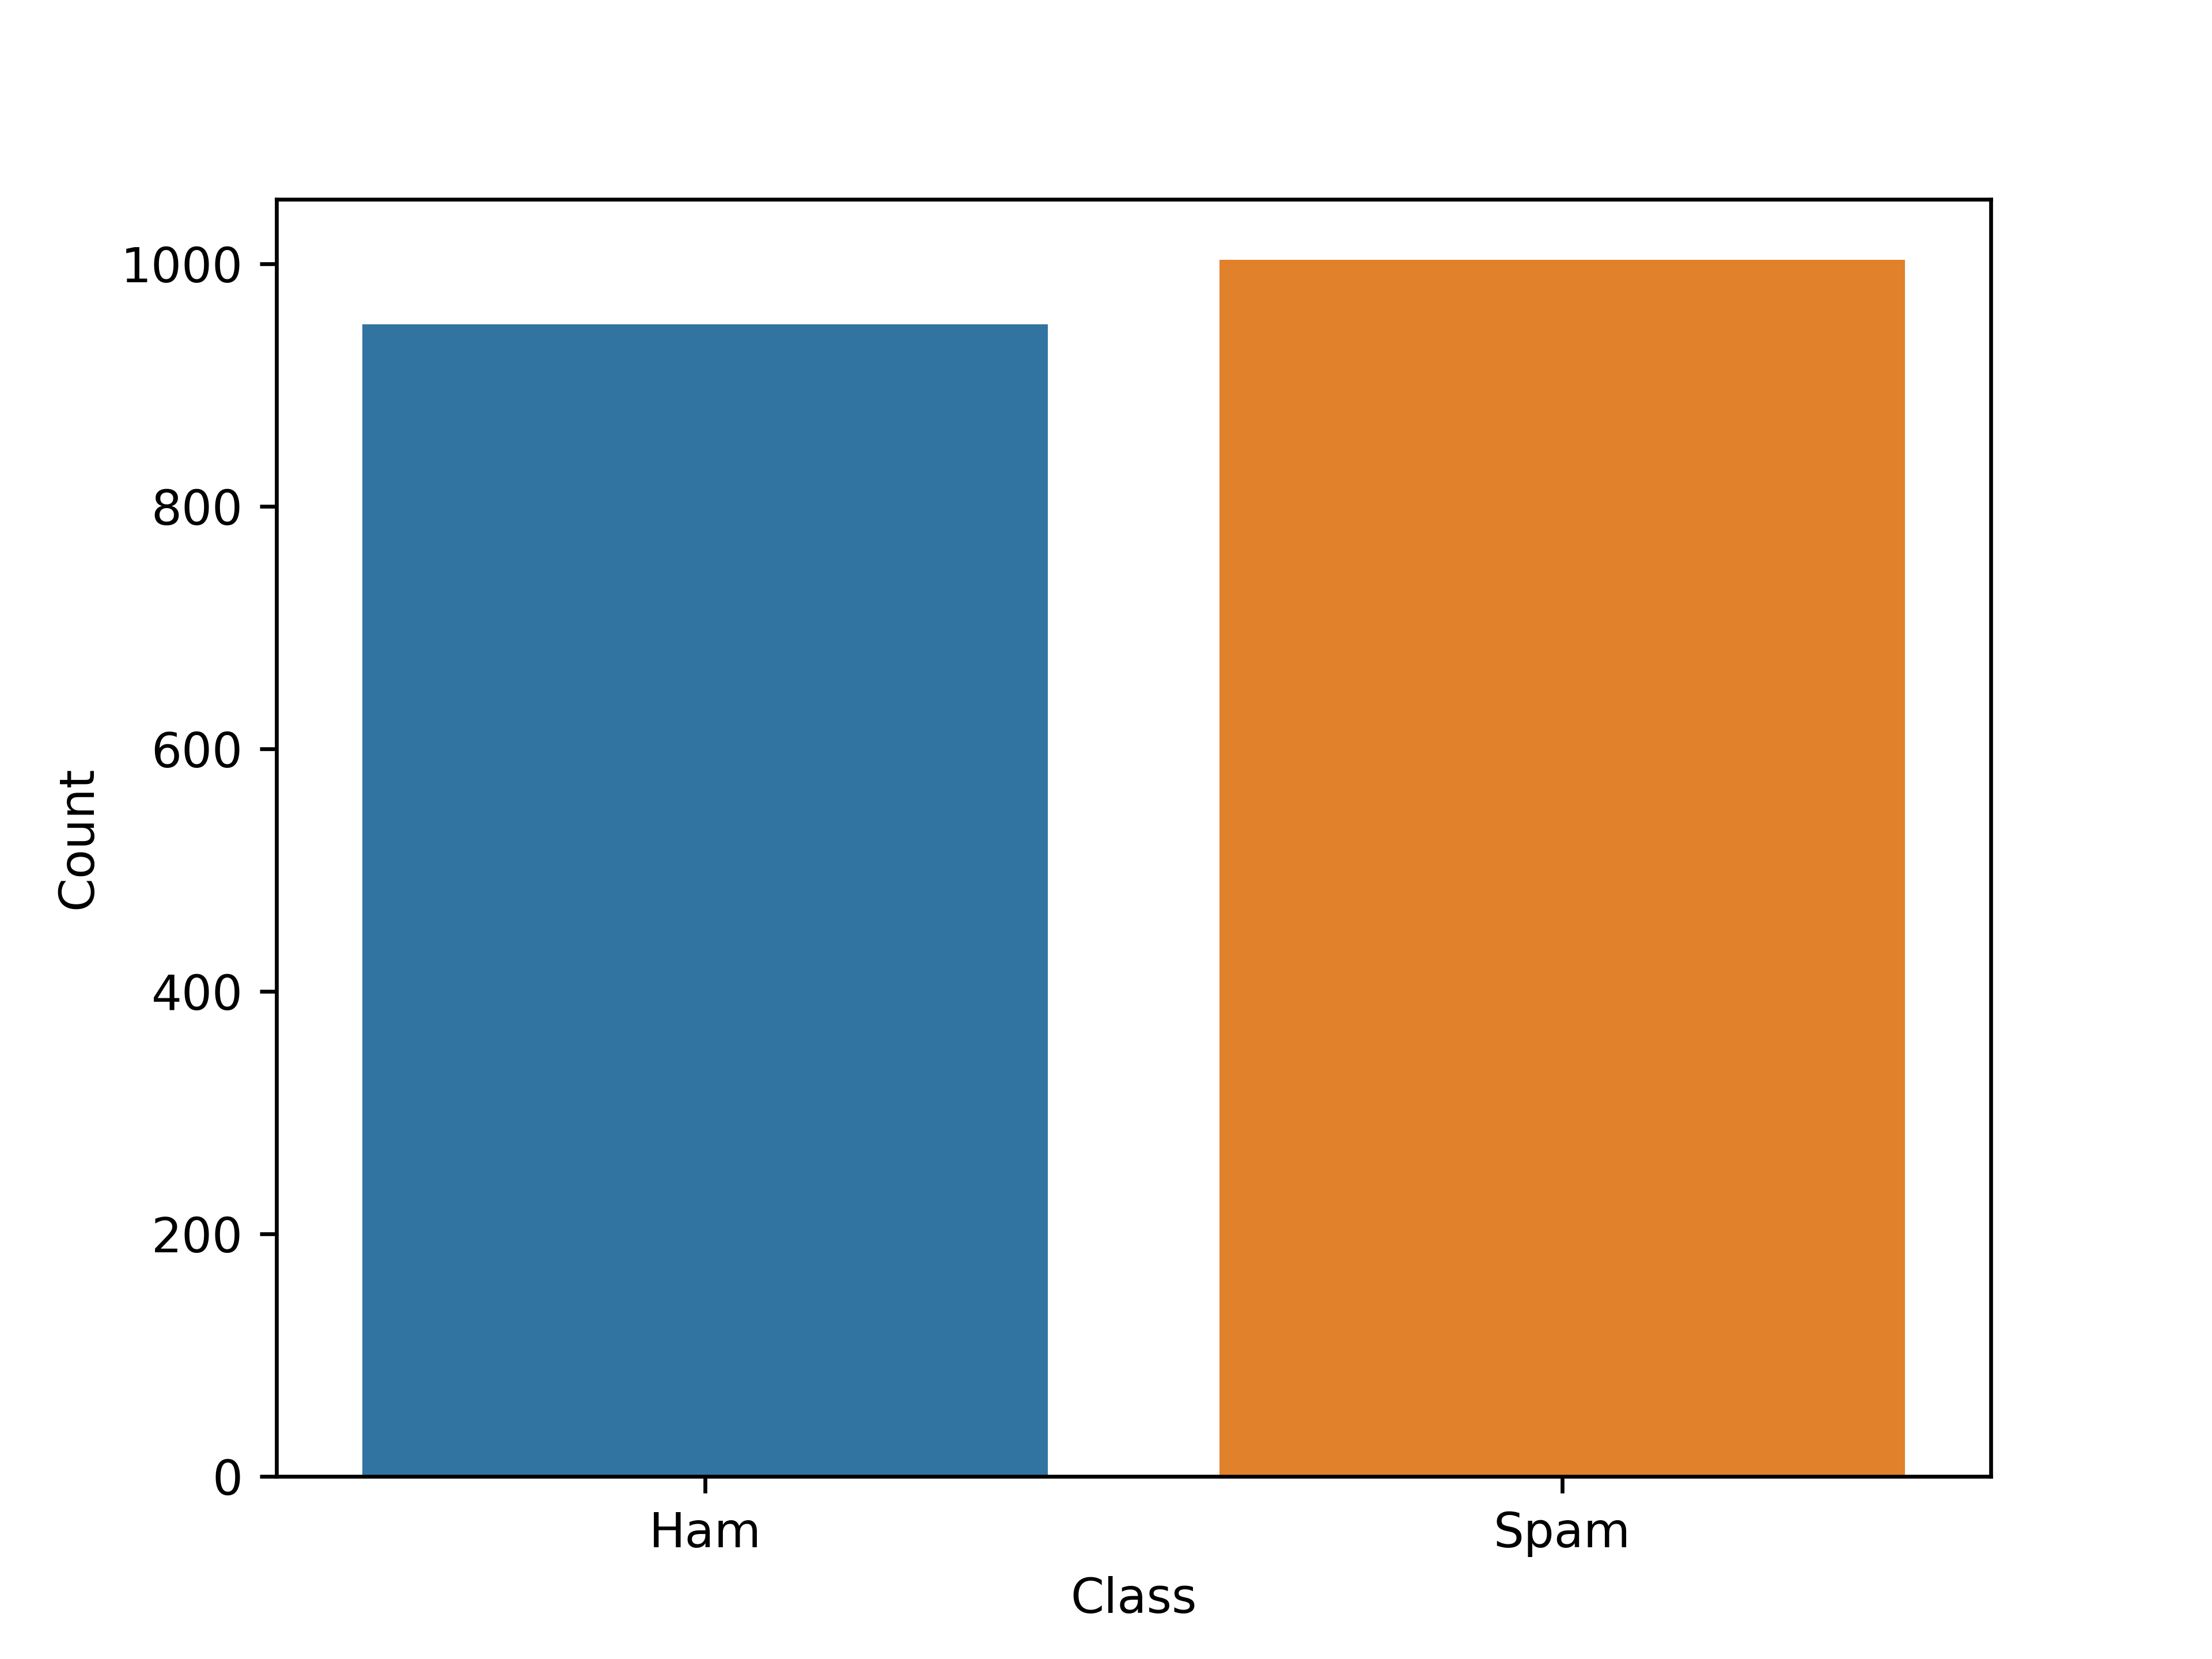
\includegraphics[width=.9\textwidth]{../src/figures/class_countplot}
\end{frame}

\section{Data preprocessing}
\begin{frame}[fragile]
	\frametitle{Cleaning}
	\begin{itemize}
		\item Checked for null values (only a few in date)
		\item Removed useless features (comment ID, author and date)
		\item Removed duplicates (only 3 duplicates, which affected the balance positively)
		\item Replaced HTML tags and entities in comments (e.g. replaced \lstinline{<br />}
		      with $\backslash$\lstinline{n})
	\end{itemize}
\end{frame}

\begin{frame}[fragile]
	\frametitle{Adding useful features}

	Tried to extract possible features that may indicate a spamming behaviour:
	\begin{itemize}
		\item Links
		\item YouTube links (spamming one's channel)
		\item Use of non-ASCII characters (e.g. emojis)
		\item Number of characters words, and sentences
		\item Number of uppercase letters
	\end{itemize}
\end{frame}

\begin{frame}
	\frametitle{Adding useful features - Links}

	Presence of links may indicate spam:

	\centering
	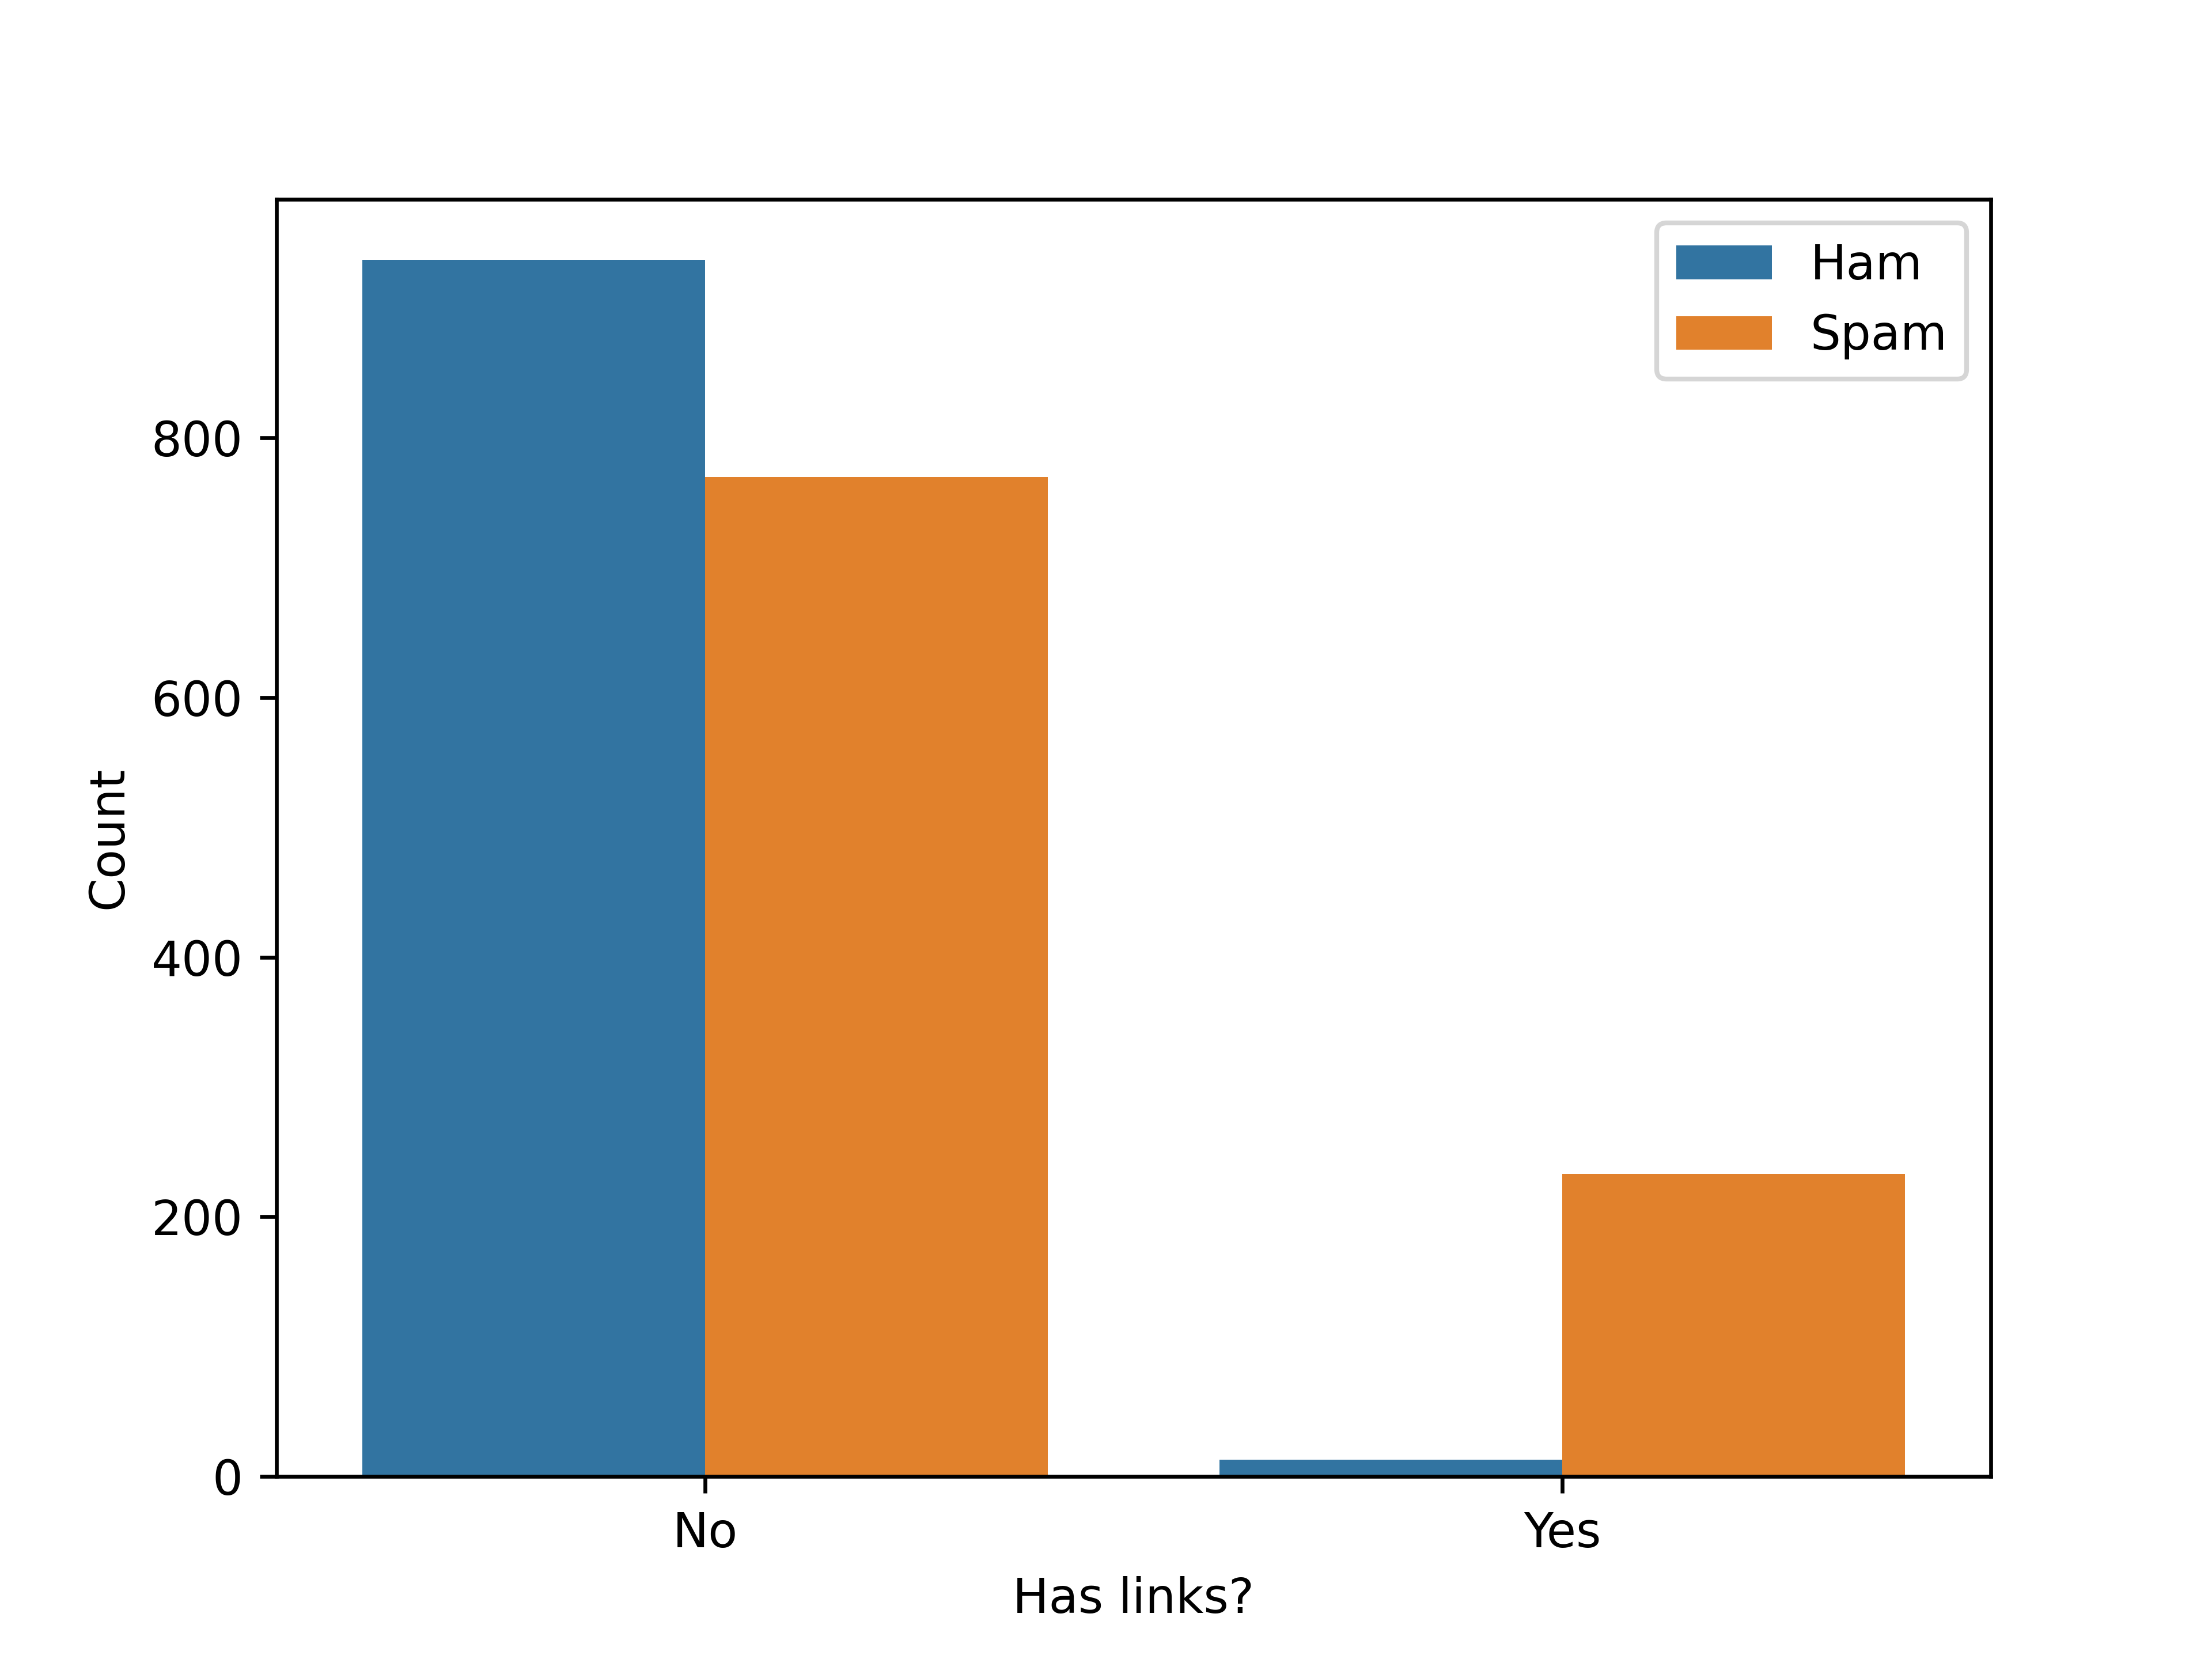
\includegraphics[width=.9\textwidth]{../src/figures/links_countplot_class}
\end{frame}

\begin{frame}
	\frametitle{Adding useful features - Characters}
	Spam comments have a much higher peak, a longer tail, and a second smaller peak at about 500 characters.
	\begin{figure}[ht]
		\begin{minipage}[b]{0.49\linewidth}
			\centering
			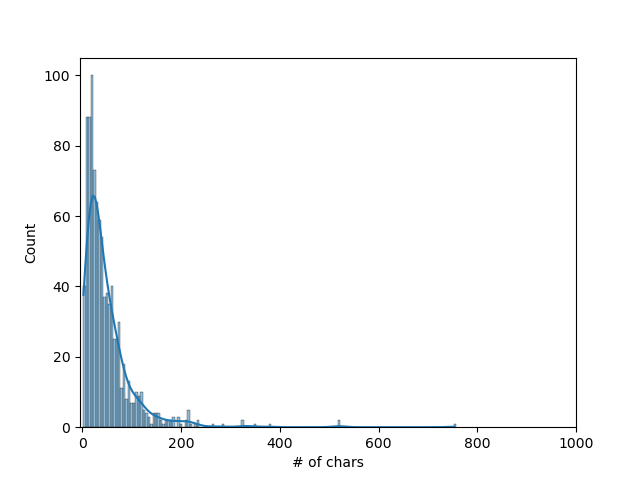
\includegraphics[width=\textwidth]{../src/figures/chars_histplot_class_0}
			\caption{Ham}
		\end{minipage}
		\begin{minipage}[b]{0.49\linewidth}
			\centering
			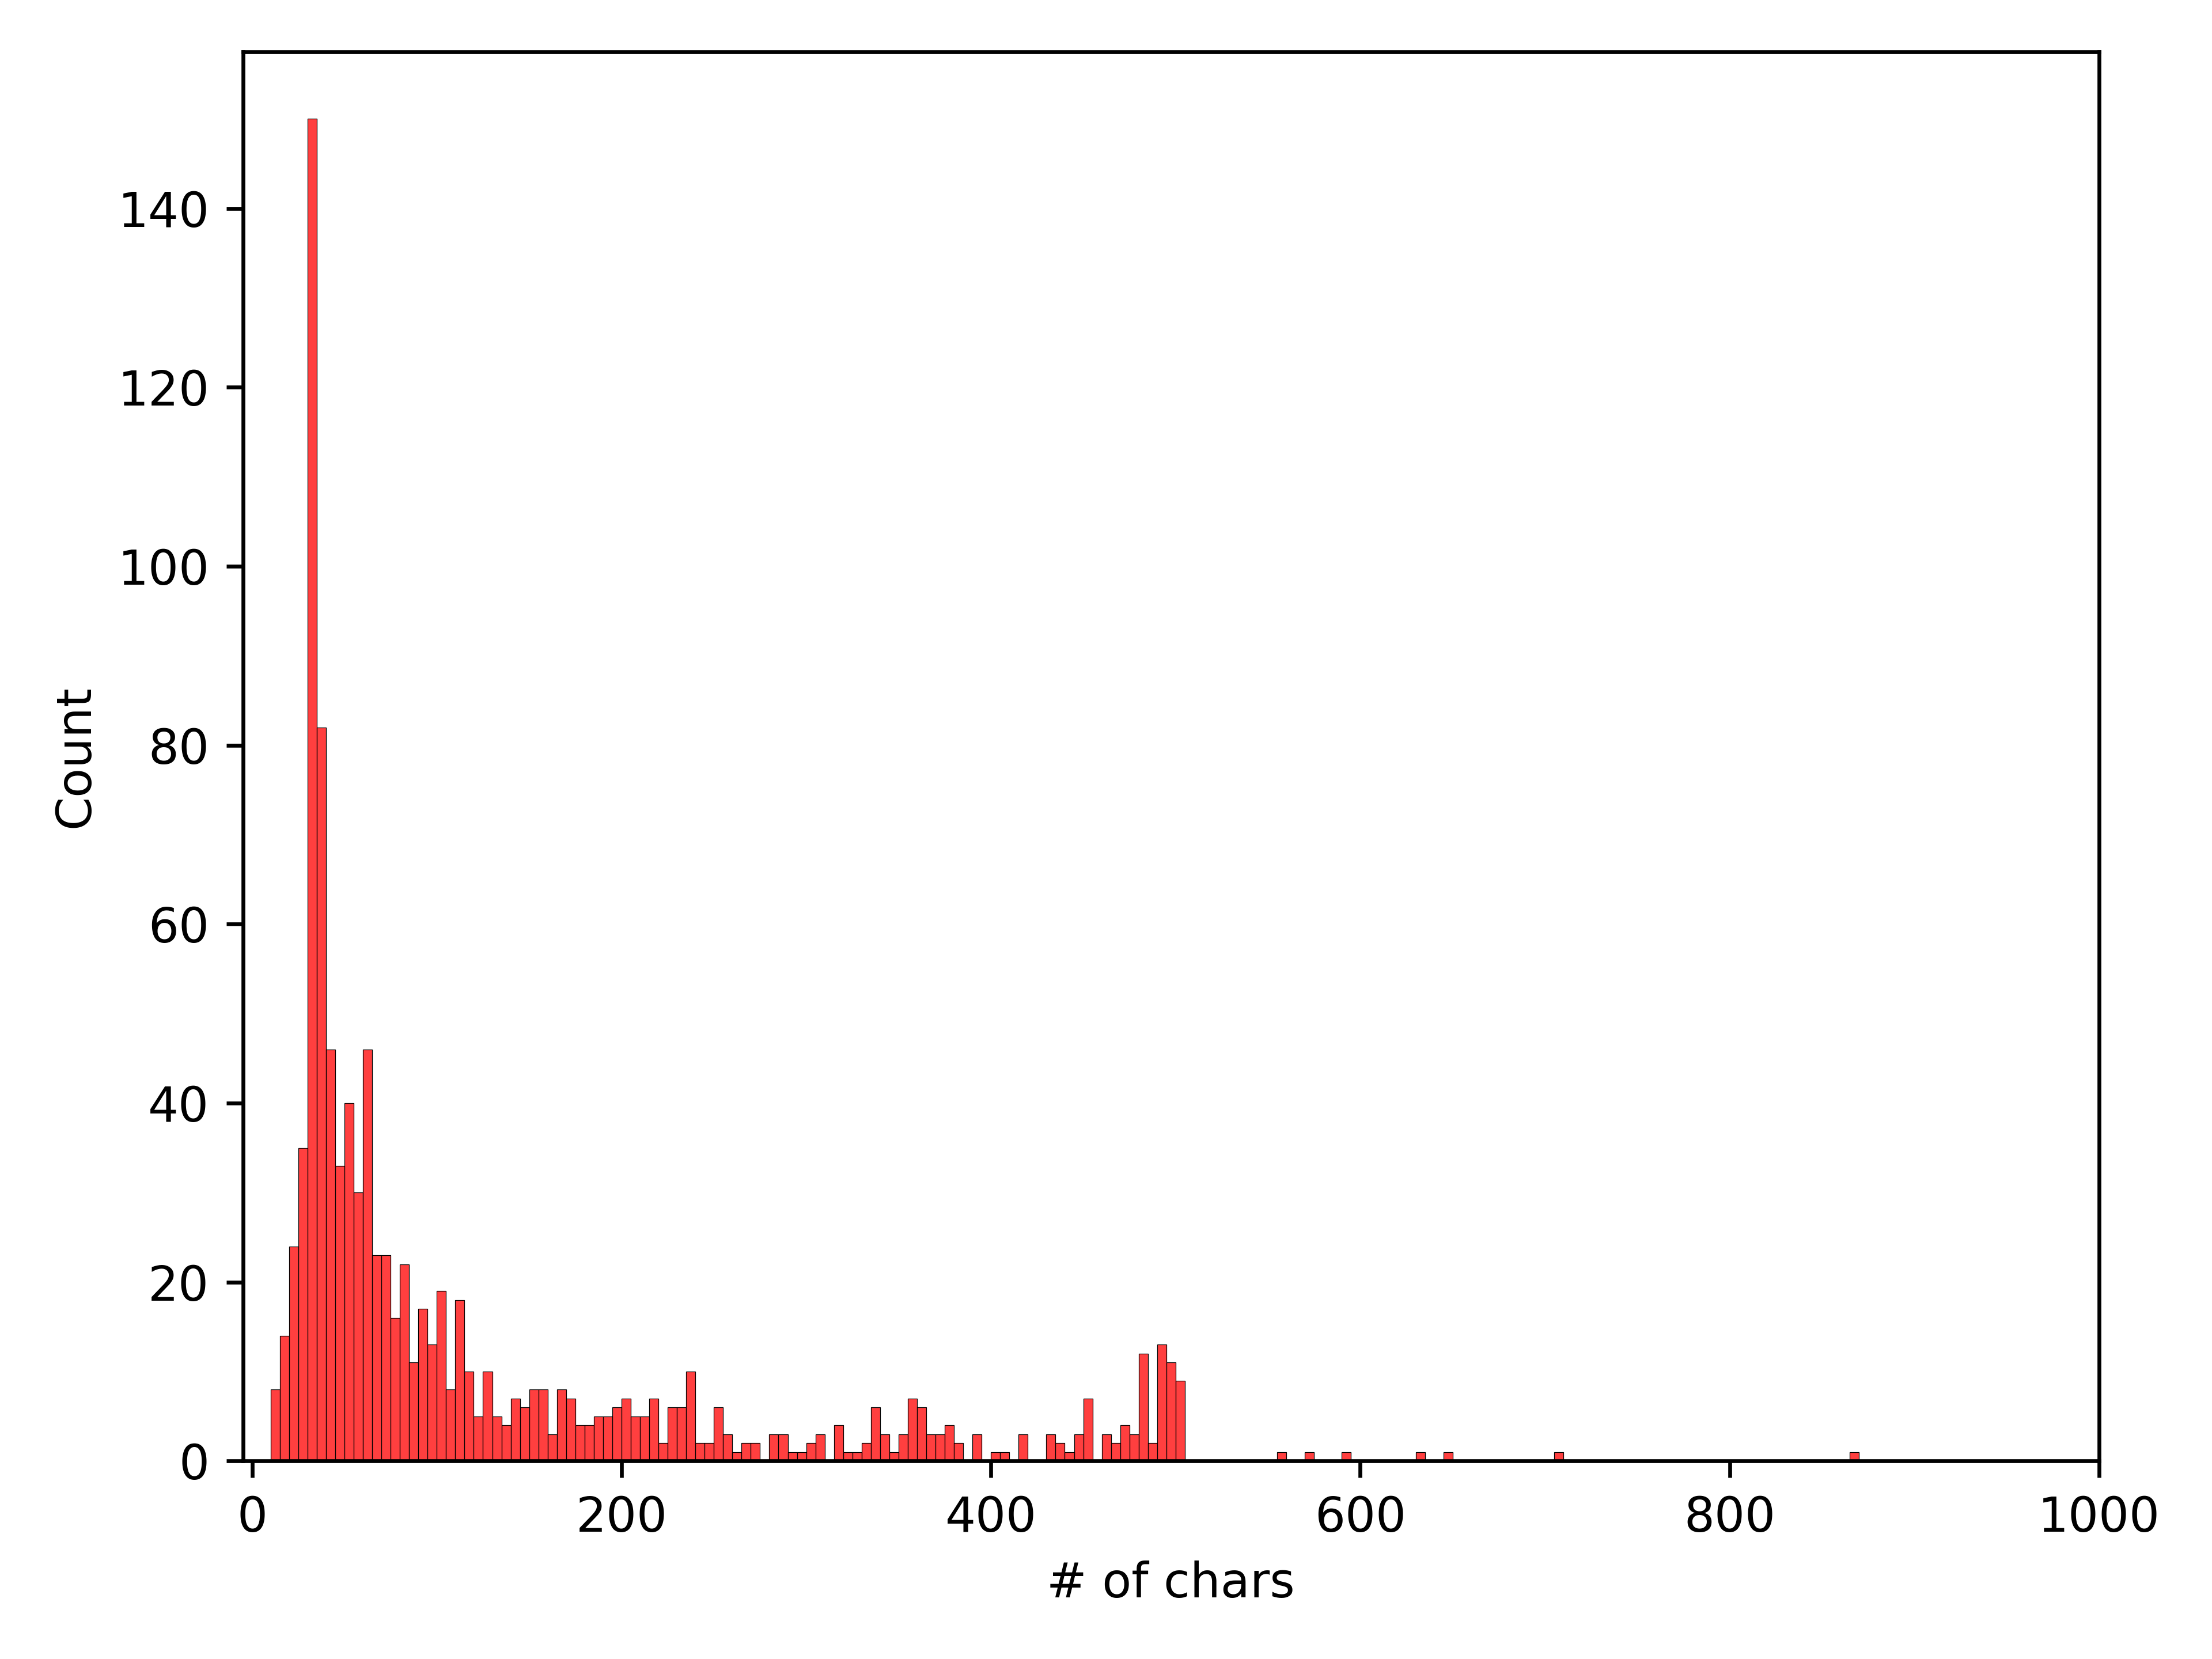
\includegraphics[width=\textwidth]{../src/figures/chars_histplot_class_1}
			\caption{Spam}
		\end{minipage}
	\end{figure}

\end{frame}

\begin{frame}
	\frametitle{Adding useful features - Heatmap}

	\centering
	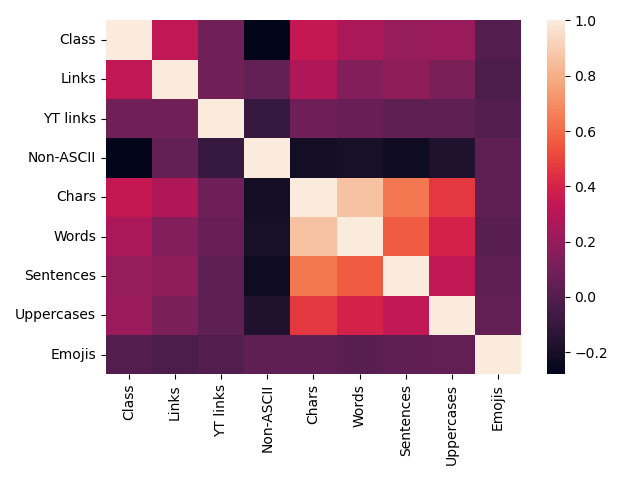
\includegraphics[width=.9\textwidth]{../src/figures/heatmap}
\end{frame}

\section{Classification}
\begin{frame}
	\frametitle{Approach}

	Classification has been performed with 4 classifiers:
	\begin{itemize}
		\item Support Vector Machine
		\item Multinomial na\"ive Bayes
		\item Decision tree
		\item Random tree
	\end{itemize}

	and with 3 different preprocessings:
	\begin{itemize}
		\item Stemming with Porter stemmer
		\item Stemming with Snowball stemmer
		\item Lemmatization
	\end{itemize}
\end{frame}

\begin{frame}
	\frametitle{Performance evaluation}
	Results obtain from K-fold (10 folds):
	\vspace{0.3cm}

	\begin{table}
		\footnotesize
		\centering
		\begin{tabular}{lcccc} \toprule
			                       & \textbf{SVM} & \textbf{Multinomial NB} & \textbf{Decision tree} & \textbf{Random forest}    \\ \cmidrule{2-5}
			\textbf{Snowball}      & 0.948        & 0.908                   & 0.957                  & \cellcolor{green!50}0.964 \\
			\textbf{Porter}        & 0.949        & 0.907                   & 0.957                  & 0.962                     \\
			\textbf{Lemmatization} & 0.947        & \cellcolor{red!50}0.903 & 0.949                  & 0.958                     \\  \bottomrule
		\end{tabular}
		\caption{F1 score}
	\end{table}
	\vspace{0.3cm}
	\begin{table}
		\footnotesize
		\centering
		\begin{tabular}{lcccc} \toprule
			                       & \textbf{SVM} & \textbf{Multinomial NB} & \textbf{Decision tree} & \textbf{Random forest}    \\\cmidrule{2-5}
			\textbf{Snowball}      & 0.948        & 0.908                   & 0.958                  & \cellcolor{green!50}0.964 \\
			\textbf{Porter}        & 0.949        & 0.907                   & 0.96                   & \cellcolor{green!50}0.964 \\
			\textbf{Lemmatization} & 0.947        & \cellcolor{red!50}0.904 & 0.949                  & 0.961                     \\ \bottomrule
		\end{tabular}
		\caption{Accuracy}
	\end{table}
\end{frame}

\begin{frame}
	\frametitle{Performance evaluation}

	\centering
	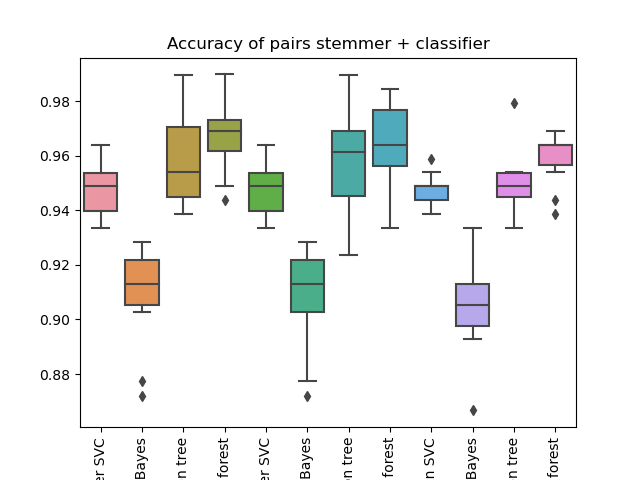
\includegraphics[width=.8\textheight]{../src/figures/boxplot_results}
\end{frame}

\begin{frame}
	\frametitle{Testing the null hypothesis}

	The random forest classifier has performed the best, whereas the preprocessing
	has a much smaller impact on final results. Wilcoxon test can be used to
	determine if there is a statistical difference between preprocessing methods
	(with a fixed classifier).

	\begin{table}
		\footnotesize
		\centering
		\begin{tabular}{cc} \toprule
			\textbf{Preprocessing pair} & \textbf{P-value} \\ \midrule
			Snowball - Porter           & 0.4962           \\
			Snowball - Lemmatization    & 0.1934           \\
			Porter - Lemmatization      & 0.1055           \\  \bottomrule
		\end{tabular}
		\caption{Random forest with different preprocessing}
	\end{table}

	Using the conventional acceptance of statistical significance at 0.05 (5\%), we
	refute the null hypothesis: \textit{the difference between the three
		proprocessing methods is not statistically significant!}
\end{frame}

\begin{frame}
	\frametitle{Performance evaluation - Other results}

	In general, Wilcoxon test allows determining that in this dataset, for the
	tested classifiers and preprocessing algorithms:
	\begin{itemize}
		\item The use of a different preprocessing is usually not significant, but it is for
		      the decision tree classifier
		\item The use of a different classifier is almost always significant
	\end{itemize}
\end{frame}

\section{Conclusions}
\begin{frame}
	\frametitle{Conclusions and future work}

	Conclusions:
	\begin{itemize}
		\item The best classifier turned out to be the Random forest model. As the classifier
		      has very good performances, the initial goal can be considered achieved
		\item The use of K-fold and of the Wilcoxon test ensure that results are
		      statistically significant
	\end{itemize}

	\pause
	Improvements/future work:
	\begin{itemize}
		\item Trying other algorithms and/or preprocessing methods, which may lead to even
		      higher performances
		\item The dataset is not large at all. To completely ensure that results can be
		      trusted, it would be needed to use a much larger dataset (possibly with at
		      least tens of thousand of comments). Unfortunately, no such dataset was found
		      online
	\end{itemize}
\end{frame}

\end{document}

